% !TEX root = ../main.tex

\chapter{Experiments}
\label{chapter:Experiments}
The goal of our experimental evaluation is to understand how the two main ideas of our algorithm contribute to its perforance in one observation, obscure goal 
POMDPs, namely the weak inductive bias as developed in \ref{COD_AC} and the inference time planning developed in \ref{inference_time_planning}. 
To do this, we first analyze our weak inductive bias against a proposed method using a recurrent architecture. 
We directly compare our results on the benchmark they provided. Second, we evaluate the perforance difference between pure imitation learning and reinforcement 
learning with expert demonstrations on the reach environment from the Meta-World benchmark. Here we compare our inference time planning against two state of 
the arts reinforcement learning algorithms, which are pretrained using behavioural cloning. For our third experiment setup, we evaluate our approach against 
baselines on 5 tasks from the Meta-World benchmark. As one observation POMDPs are not well studied, we propose a variety of  
baselines aiming to challenge aspects we developed in our methodology.


\section{Imitation Learning}
In this section we present our findings on the natural language conditioned robot manipulation task benchmark, that was propsed by Simon Stepputtis et.al 
\cite{stepputtis2020languageconditioned}. The benchmark consists of a 7 dof simulated robot arm with a table-top setup using CoppeliaSim which allows 
for accurate dynamics simulations at an update rate of 20Hz. The task is to pick up the correct cup and pour the content into the correct bowl, using 
natural language description of the cup and bowl and an RGB picture of the scene.\\
Three differently colored cups containing a granular material which could be poured into the bowls were used. For the bowls, 20 variations of in two sizes, 
two shape types, and five colors are used.\\
Successful picking action involved lifting a grasped object stably from the table, while successful pouring was detected whenever the cup's dispersed 
content ended up in the correct bowl. A random subset of objects was placed on the table, with a constraint to prevent collisions or other artifacts. 

Fig. 2 depicts the table-top setup and the different variations of the objects used.

As stated in section \ref{LCILRM}, in this experiment only the first observation consisting of the RGB values from the picture of the scene and the 
task description is visible for the actor. With this setup we want to evaluate our positional encoding bias. The method proposed in the accompanying 
paper "Language-Conditioned Imitation Learning for Robot Manipulation Tasks" uses a recurrent policy. As we have motivated in section \ref{COD_AC}, 
we expect our method to perform better then autoregressive or recurrent models, because we use the knowledge that we are not getting additional information 
from the environment during the unroll of the trajectory. To test this, we have used the dataset of 40000 expert demonstrations provided 
with the benchmark to train our model using only imitation learning. 

The results are depicted in table

On the 100 test environments that were provided, we decreased the overall error rate by 97$ \% $. 
\begin{figure}
    \captionsetup[subfigure]{justification=Centering, labelformat=empty}
    \begin{subfigure}[t]{0.18\textwidth}
        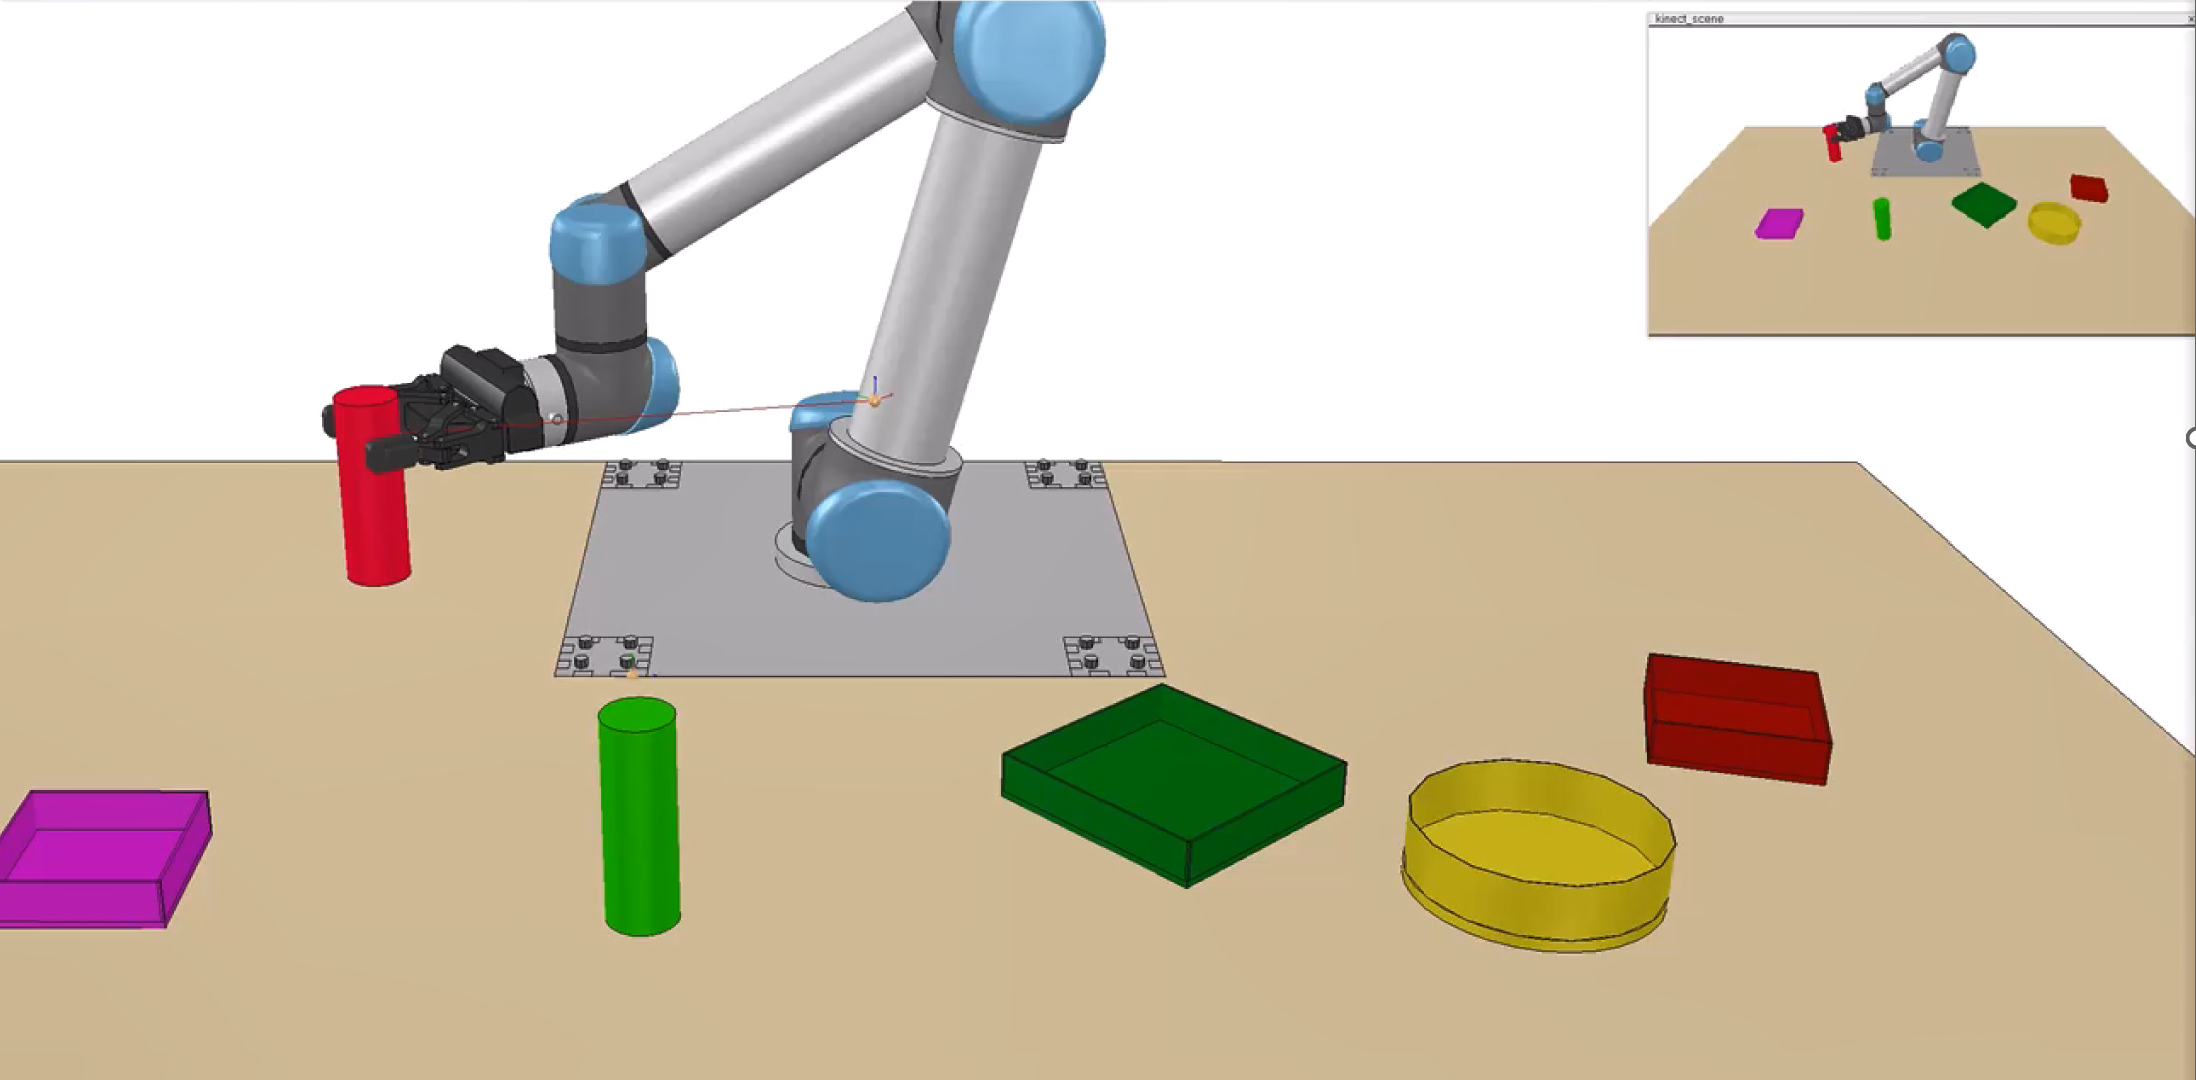
\includegraphics[width=\textwidth]{images/Language_Conditioned_Exp/theirs_1.png}
        \caption{Time step 60.}
    \end{subfigure}
    \begin{subfigure}[t]{0.18\textwidth}
        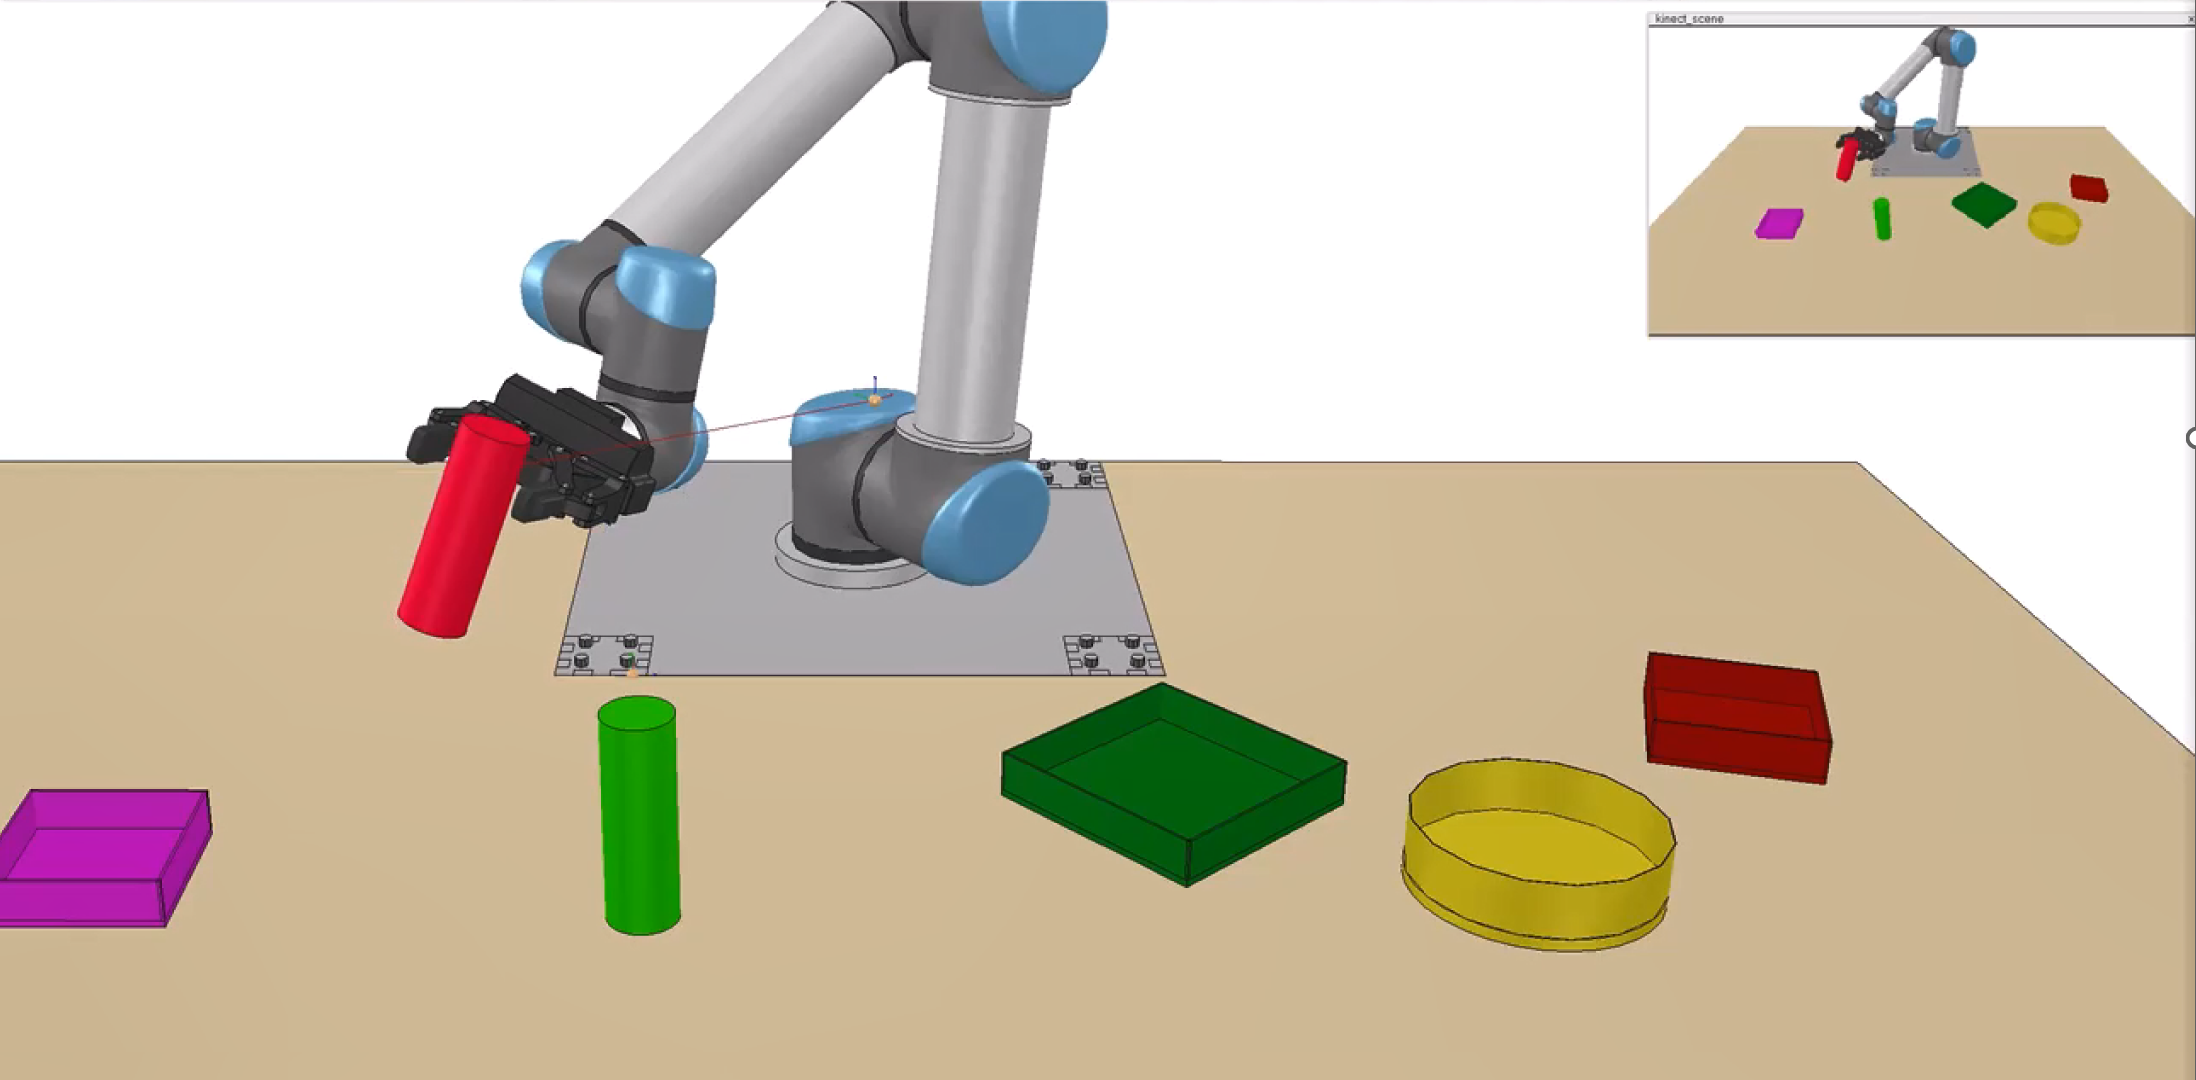
\includegraphics[width=\linewidth]{images/Language_Conditioned_Exp/theirs_2.png}
        \caption{Time step 120.}
    \end{subfigure}
    \begin{subfigure}[t]{0.18\textwidth}
        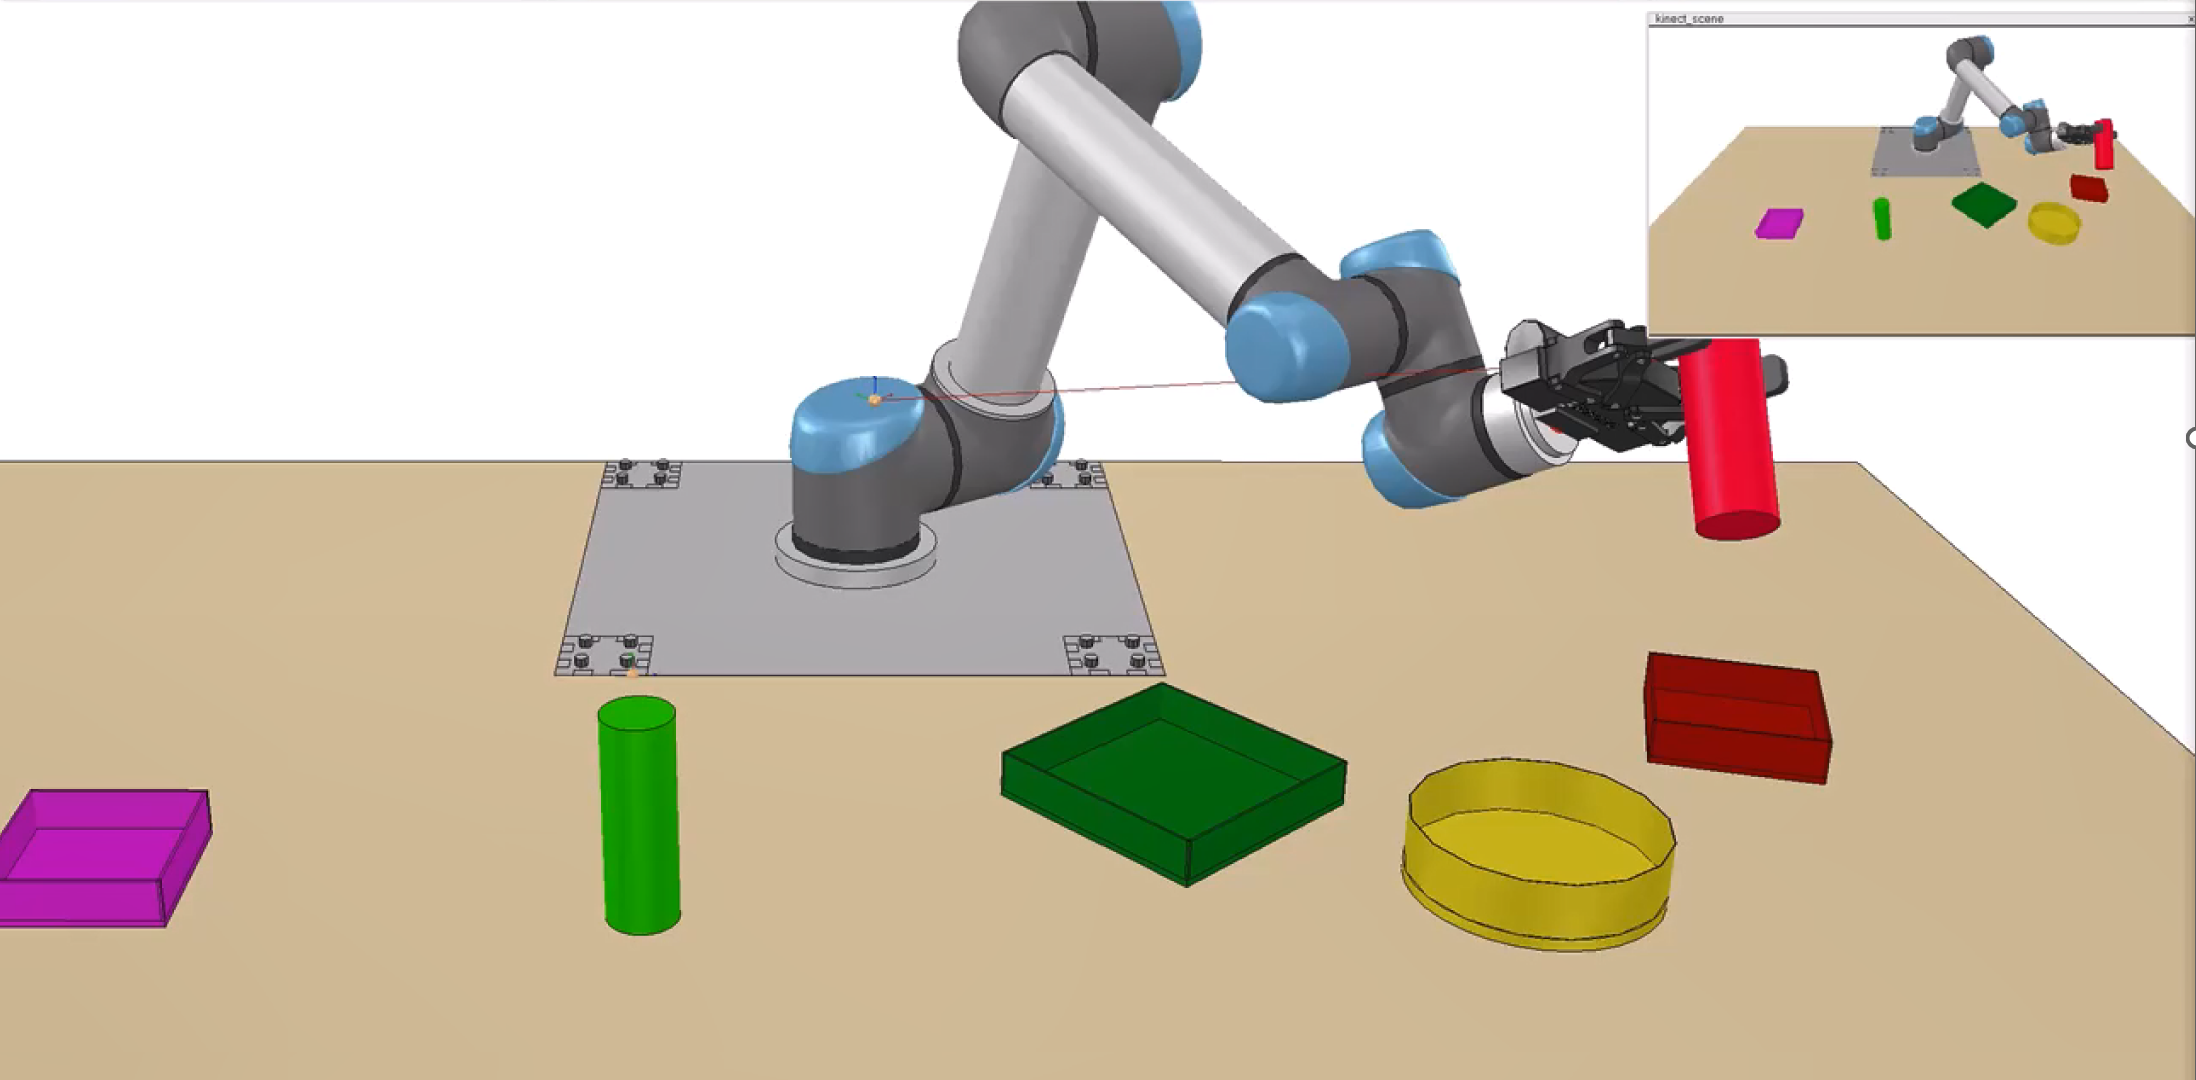
\includegraphics[width=\linewidth]{images/Language_Conditioned_Exp/theirs_3.png}
        \caption{Time step 180.}
    \end{subfigure}
    \begin{subfigure}[t]{0.18\textwidth}
        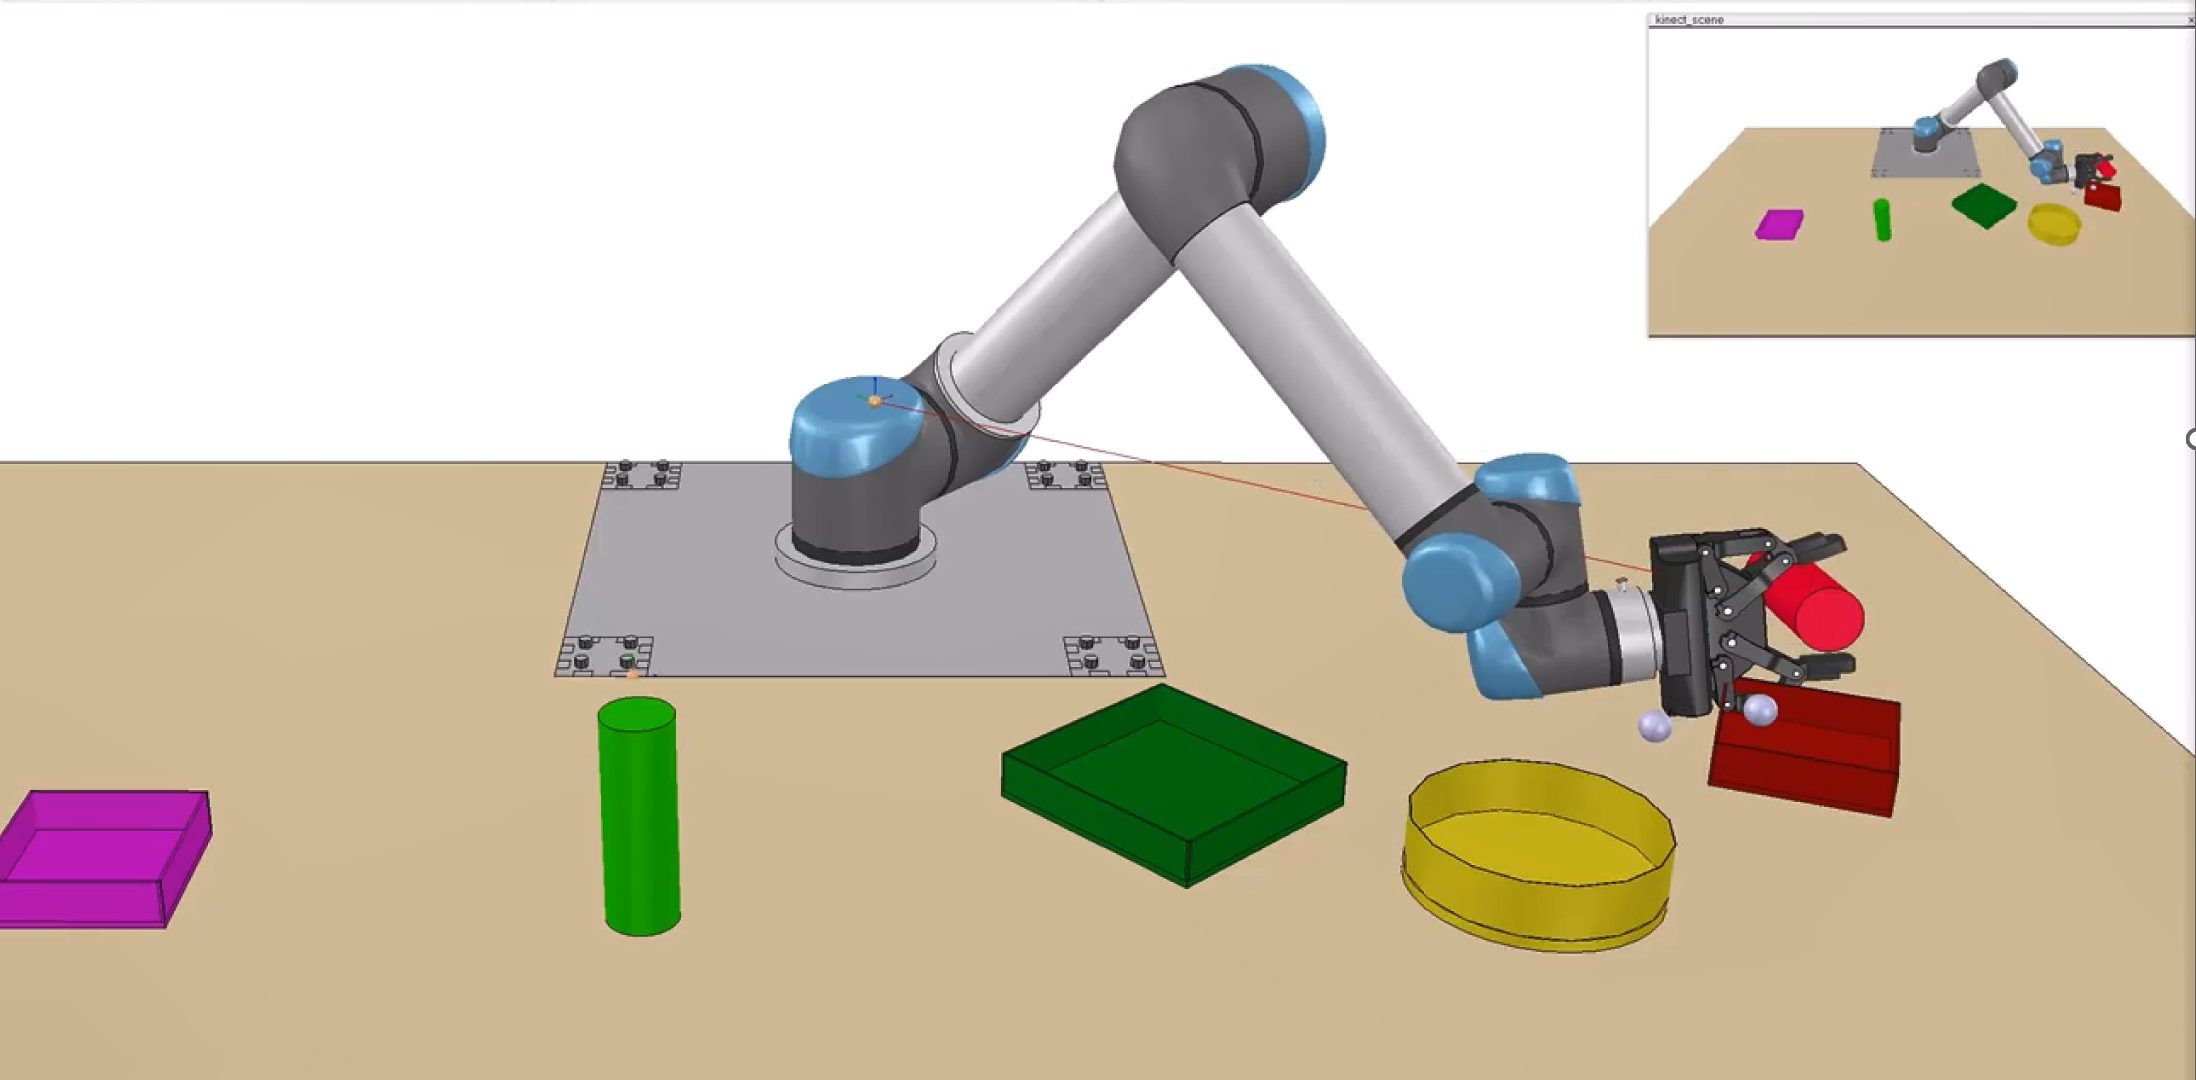
\includegraphics[width=\linewidth]{images/Language_Conditioned_Exp/theirs_4.png}
        \caption{Time step 240.}
    \end{subfigure}
    \begin{subfigure}[t]{0.18\textwidth}
        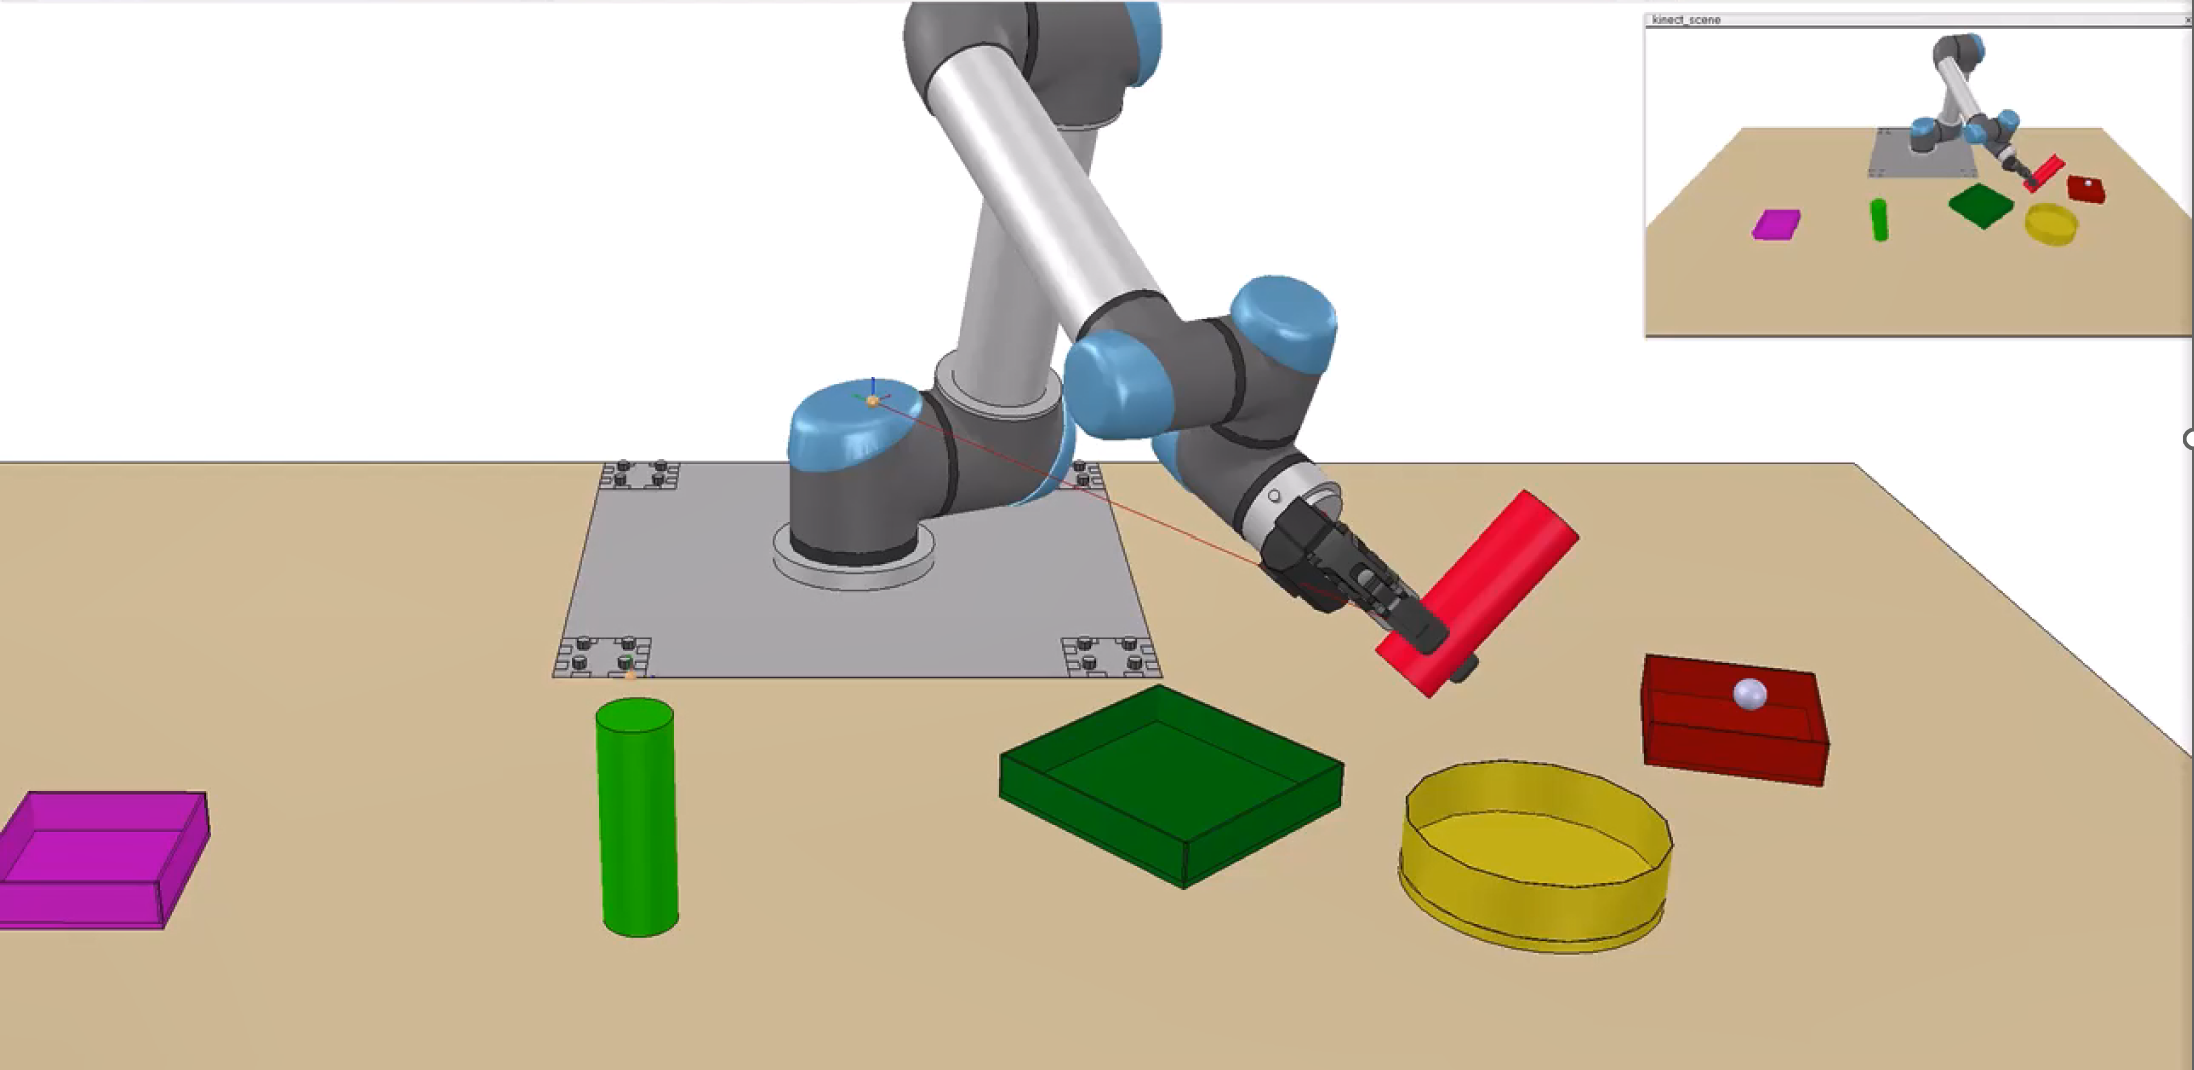
\includegraphics[width=\linewidth]{images/Language_Conditioned_Exp/theirs_5.png}
        \caption{Time step 300.}
    \end{subfigure}

    \bigskip % more vertical separation
    \begin{subfigure}[t]{0.18\textwidth}
        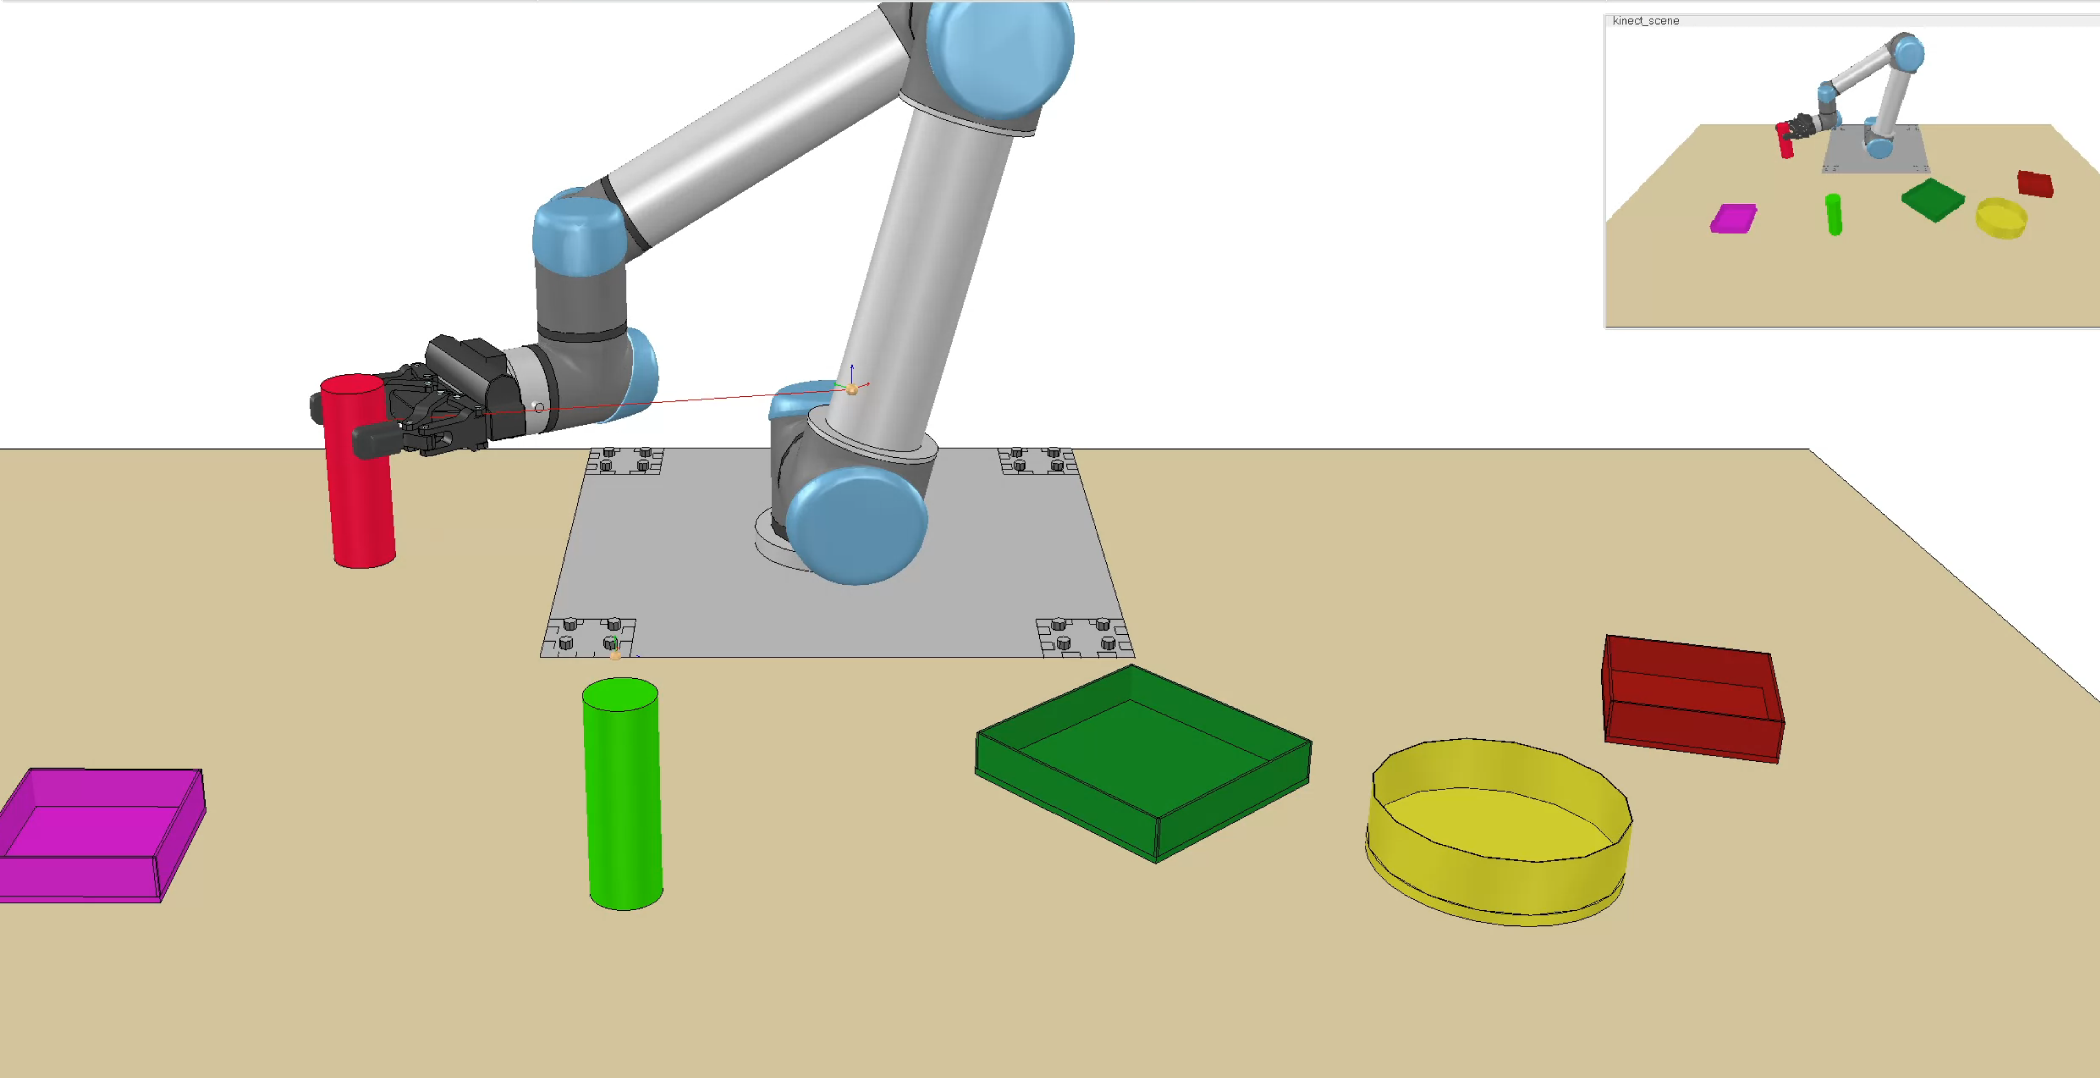
\includegraphics[width=\linewidth]{images/Language_Conditioned_Exp/mine_1.png}
        \caption{Time step 60.}
    \end{subfigure}
    \begin{subfigure}[t]{0.18\textwidth}
        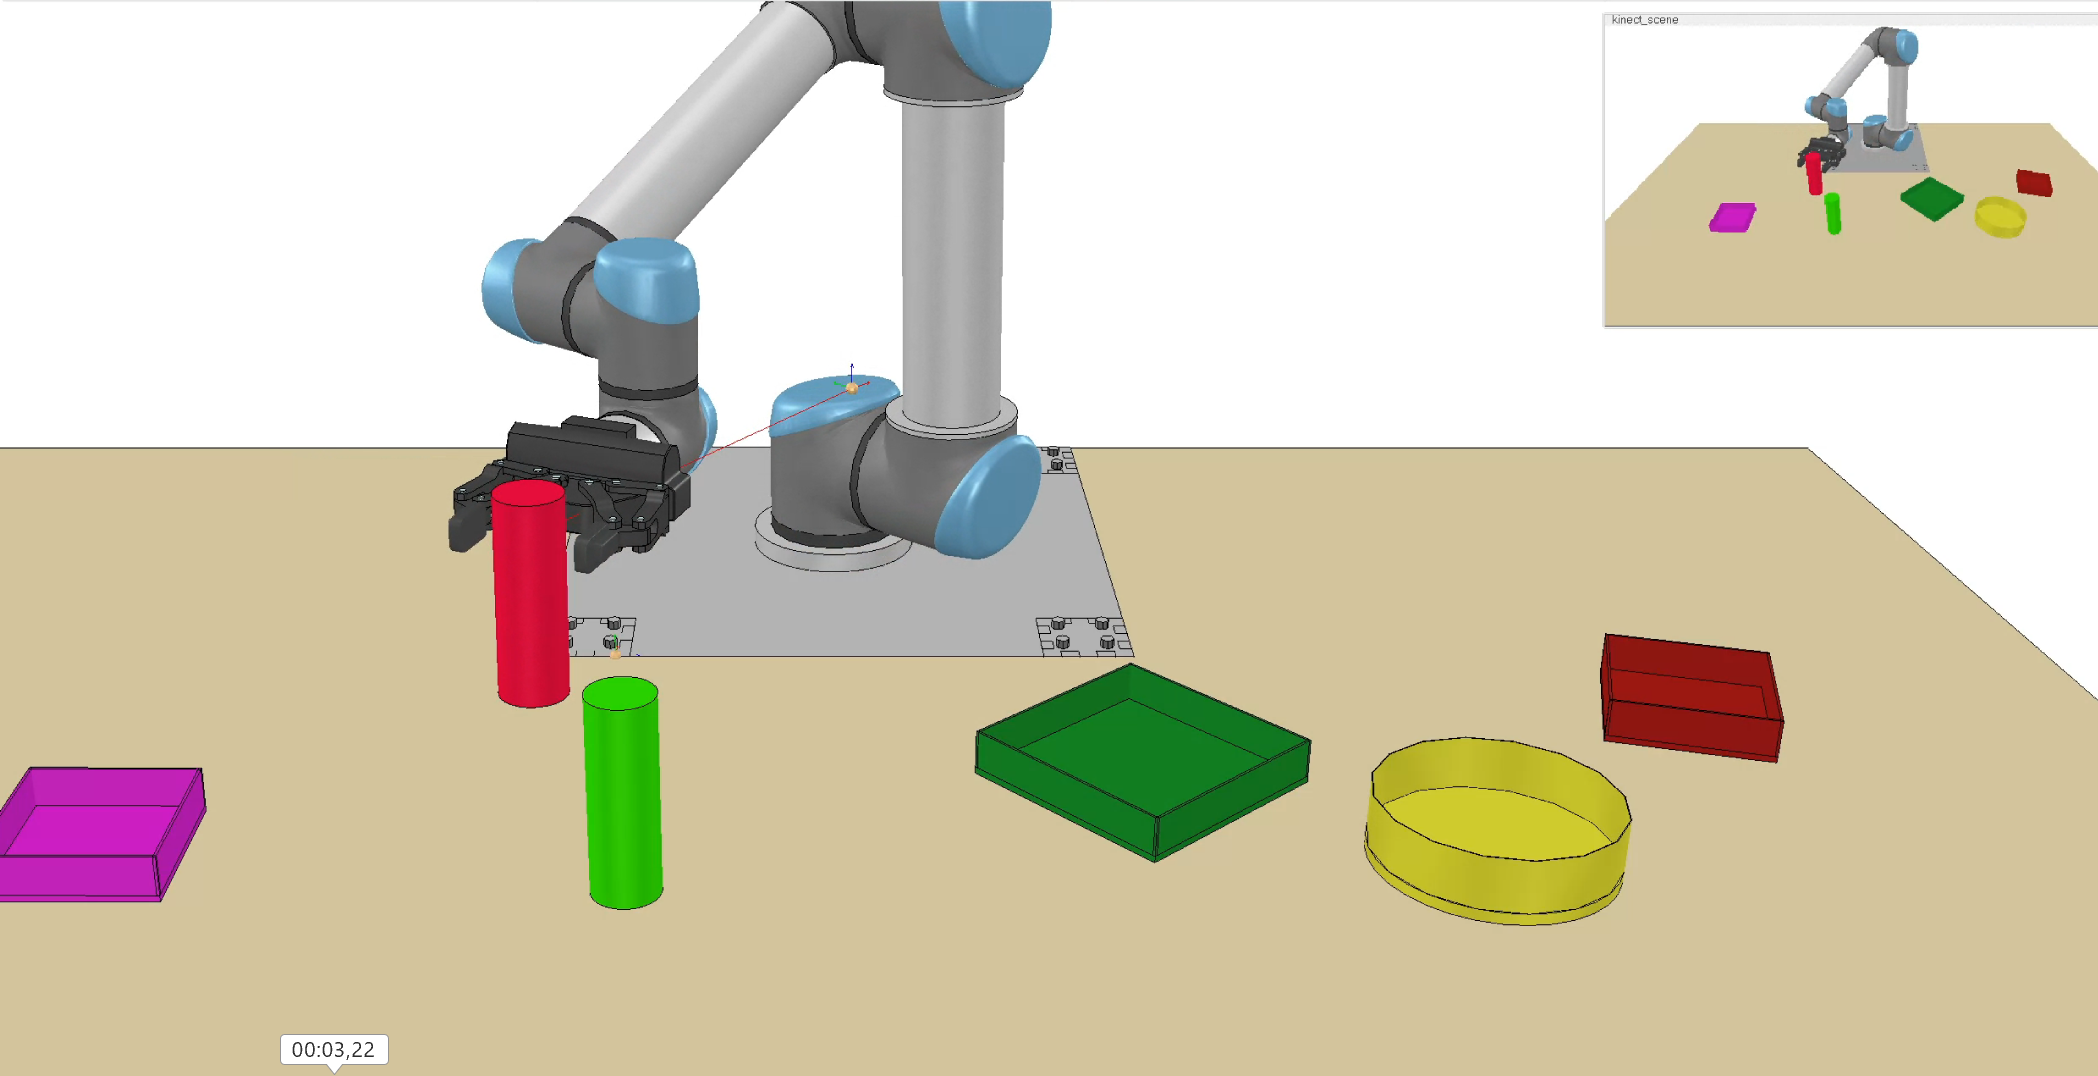
\includegraphics[width=\linewidth]{images/Language_Conditioned_Exp/mine_2.png}
        \caption{Time step 120.}
    \end{subfigure}
    \begin{subfigure}[t]{0.18\textwidth}
        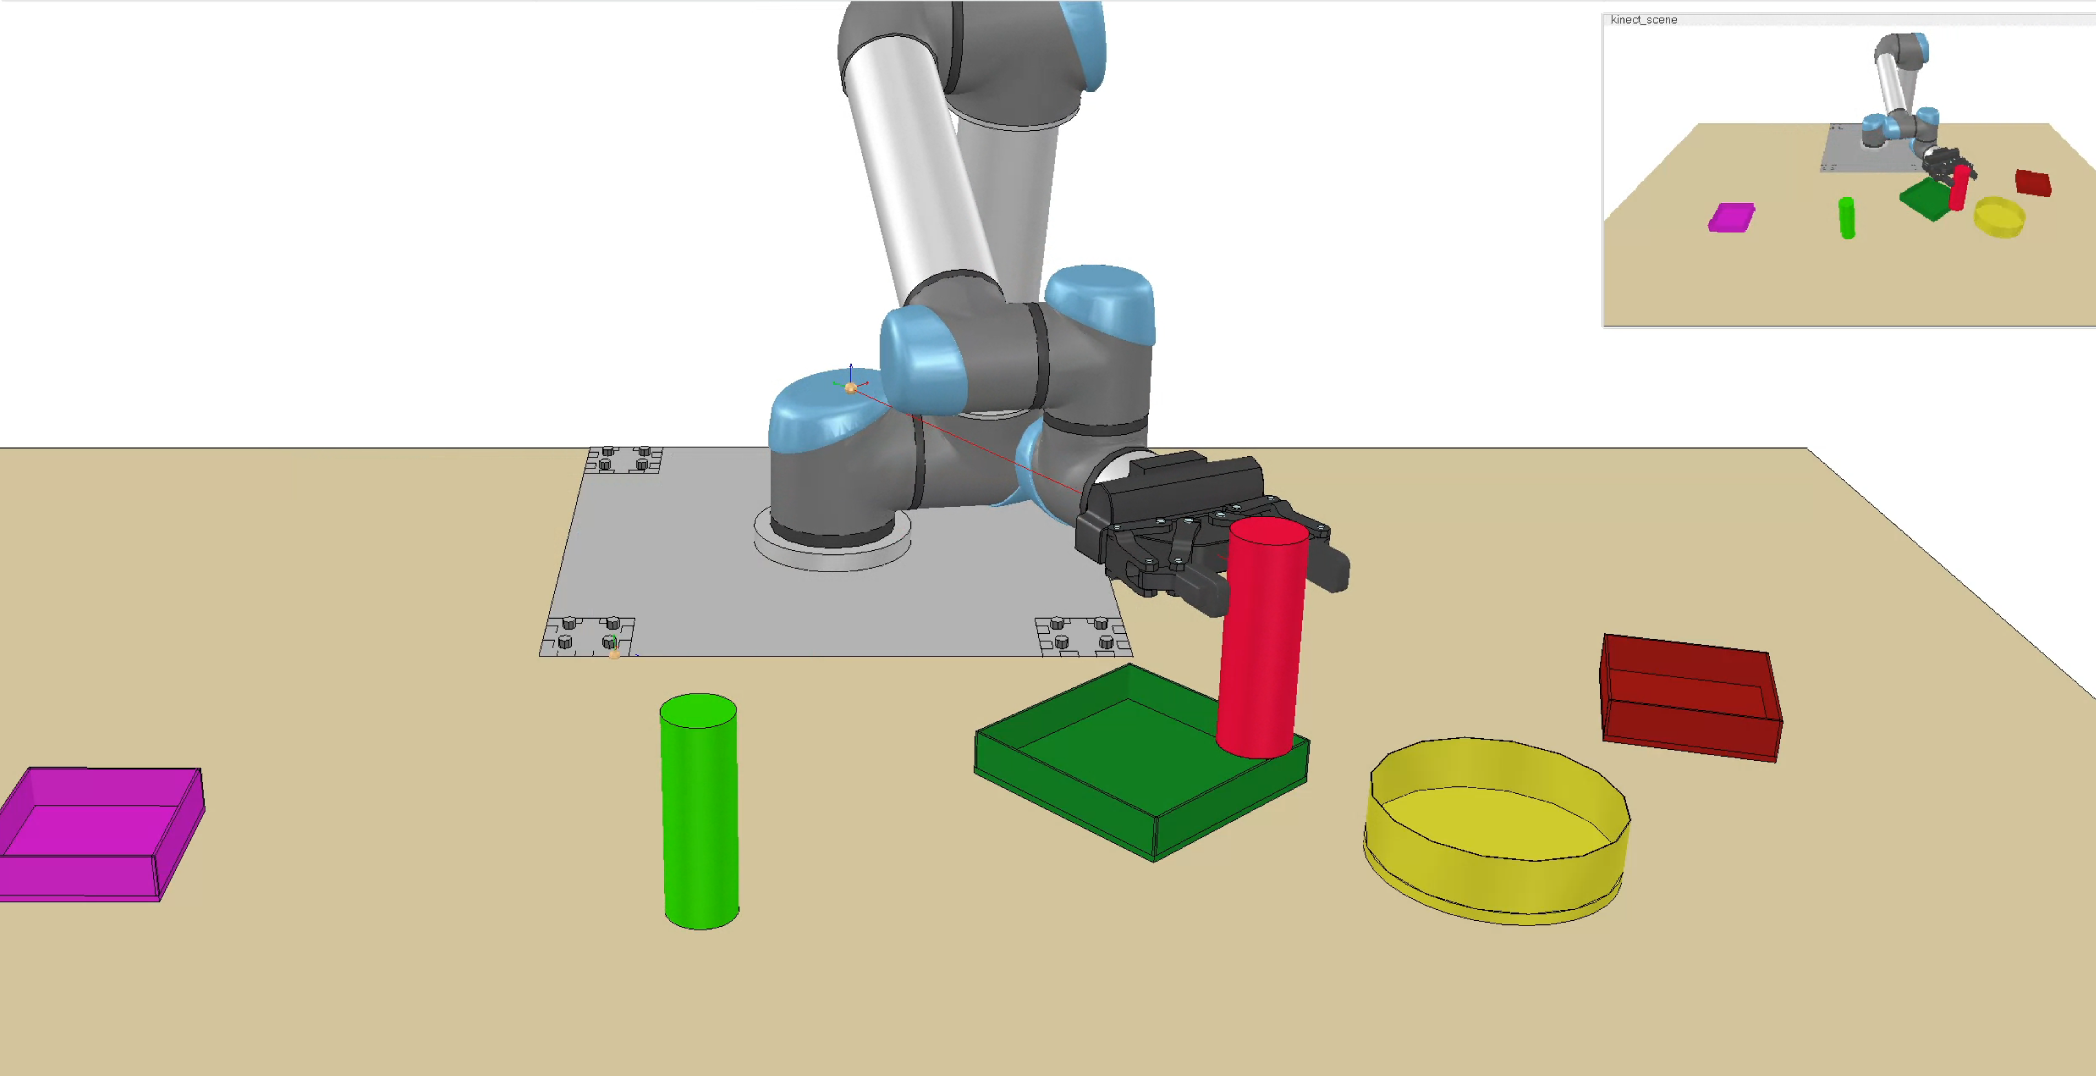
\includegraphics[width=\linewidth]{images/Language_Conditioned_Exp/mine_3.png}
        \caption{Time step 180.}
    \end{subfigure}
    \begin{subfigure}[t]{0.18\textwidth}
        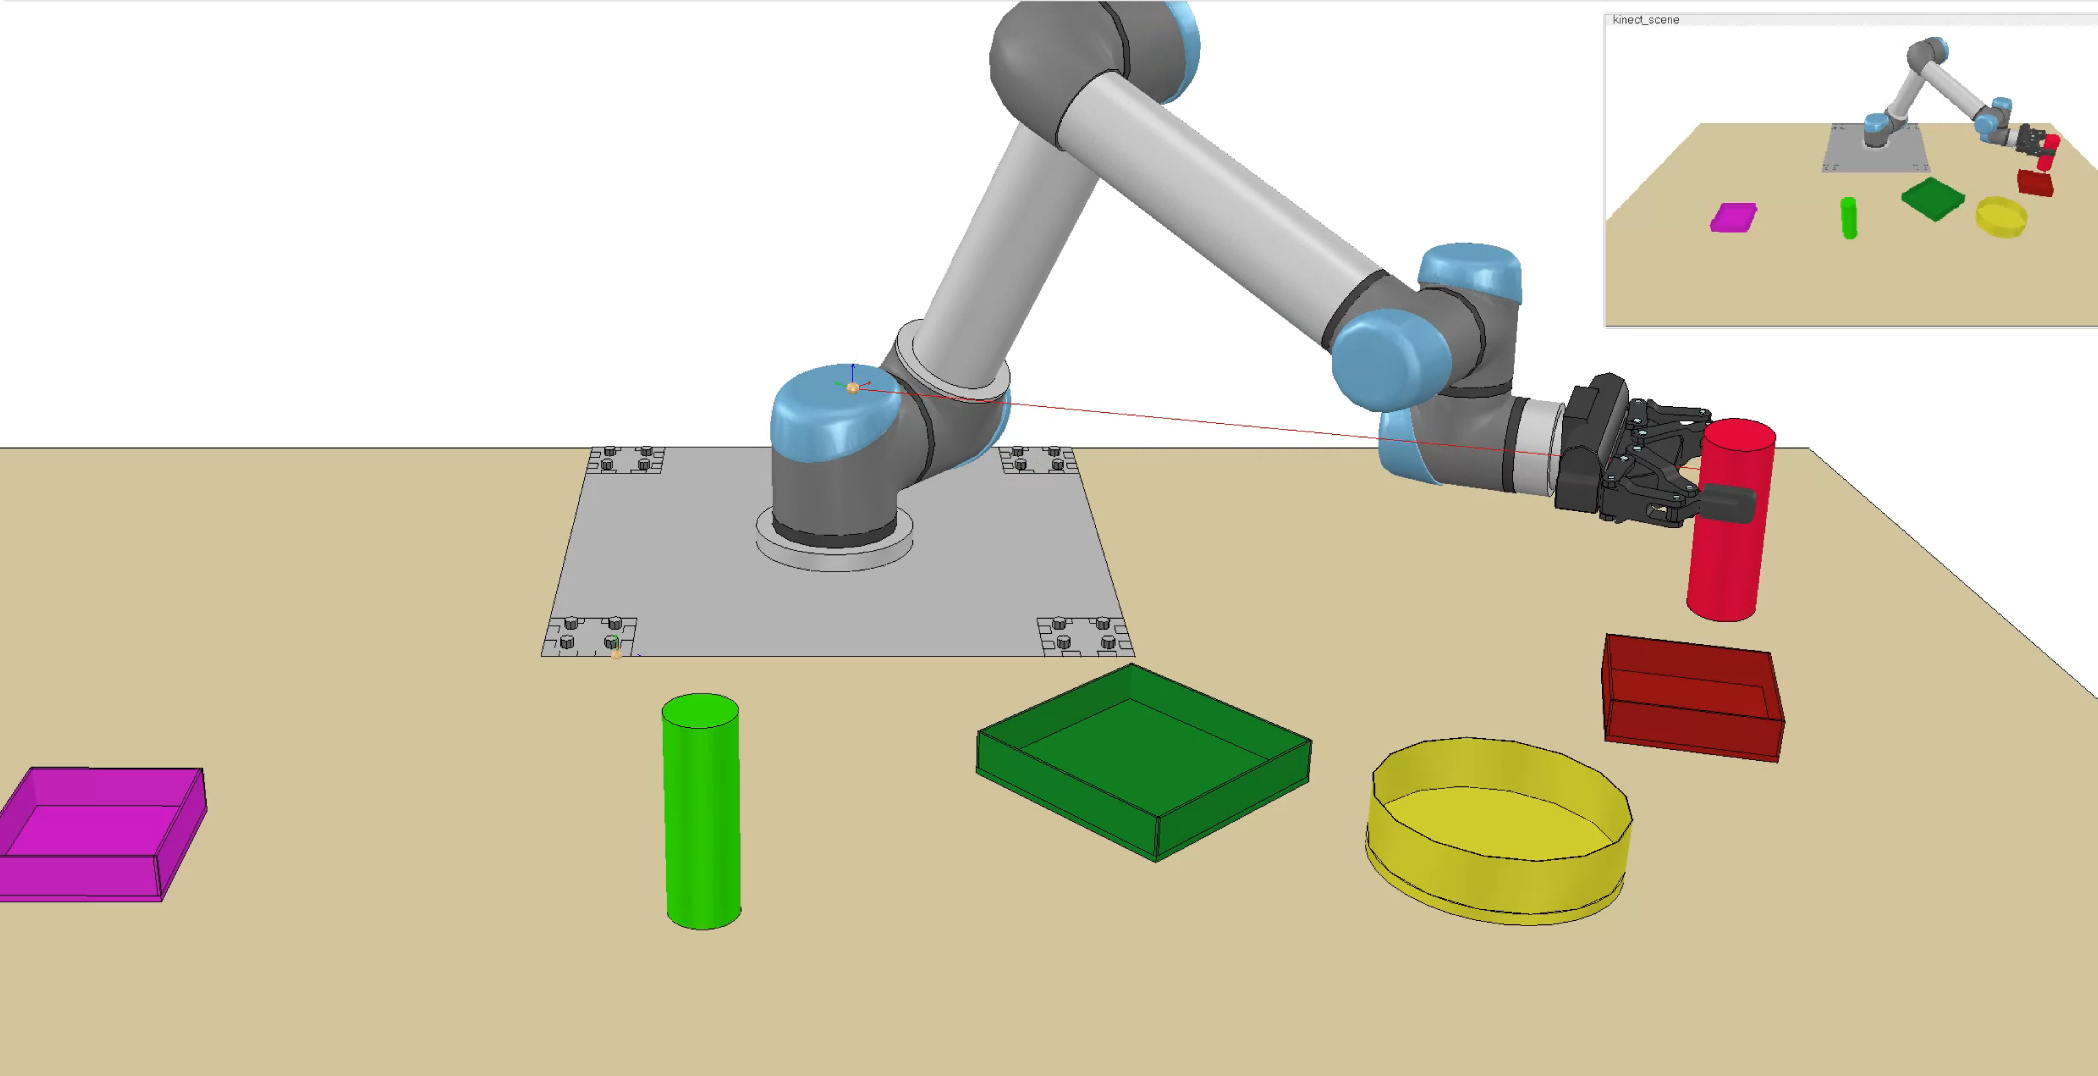
\includegraphics[width=\linewidth]{images/Language_Conditioned_Exp/mine_4.png}
        \caption{Time step 240.}
    \end{subfigure}
    \begin{subfigure}[t]{0.18\textwidth}
        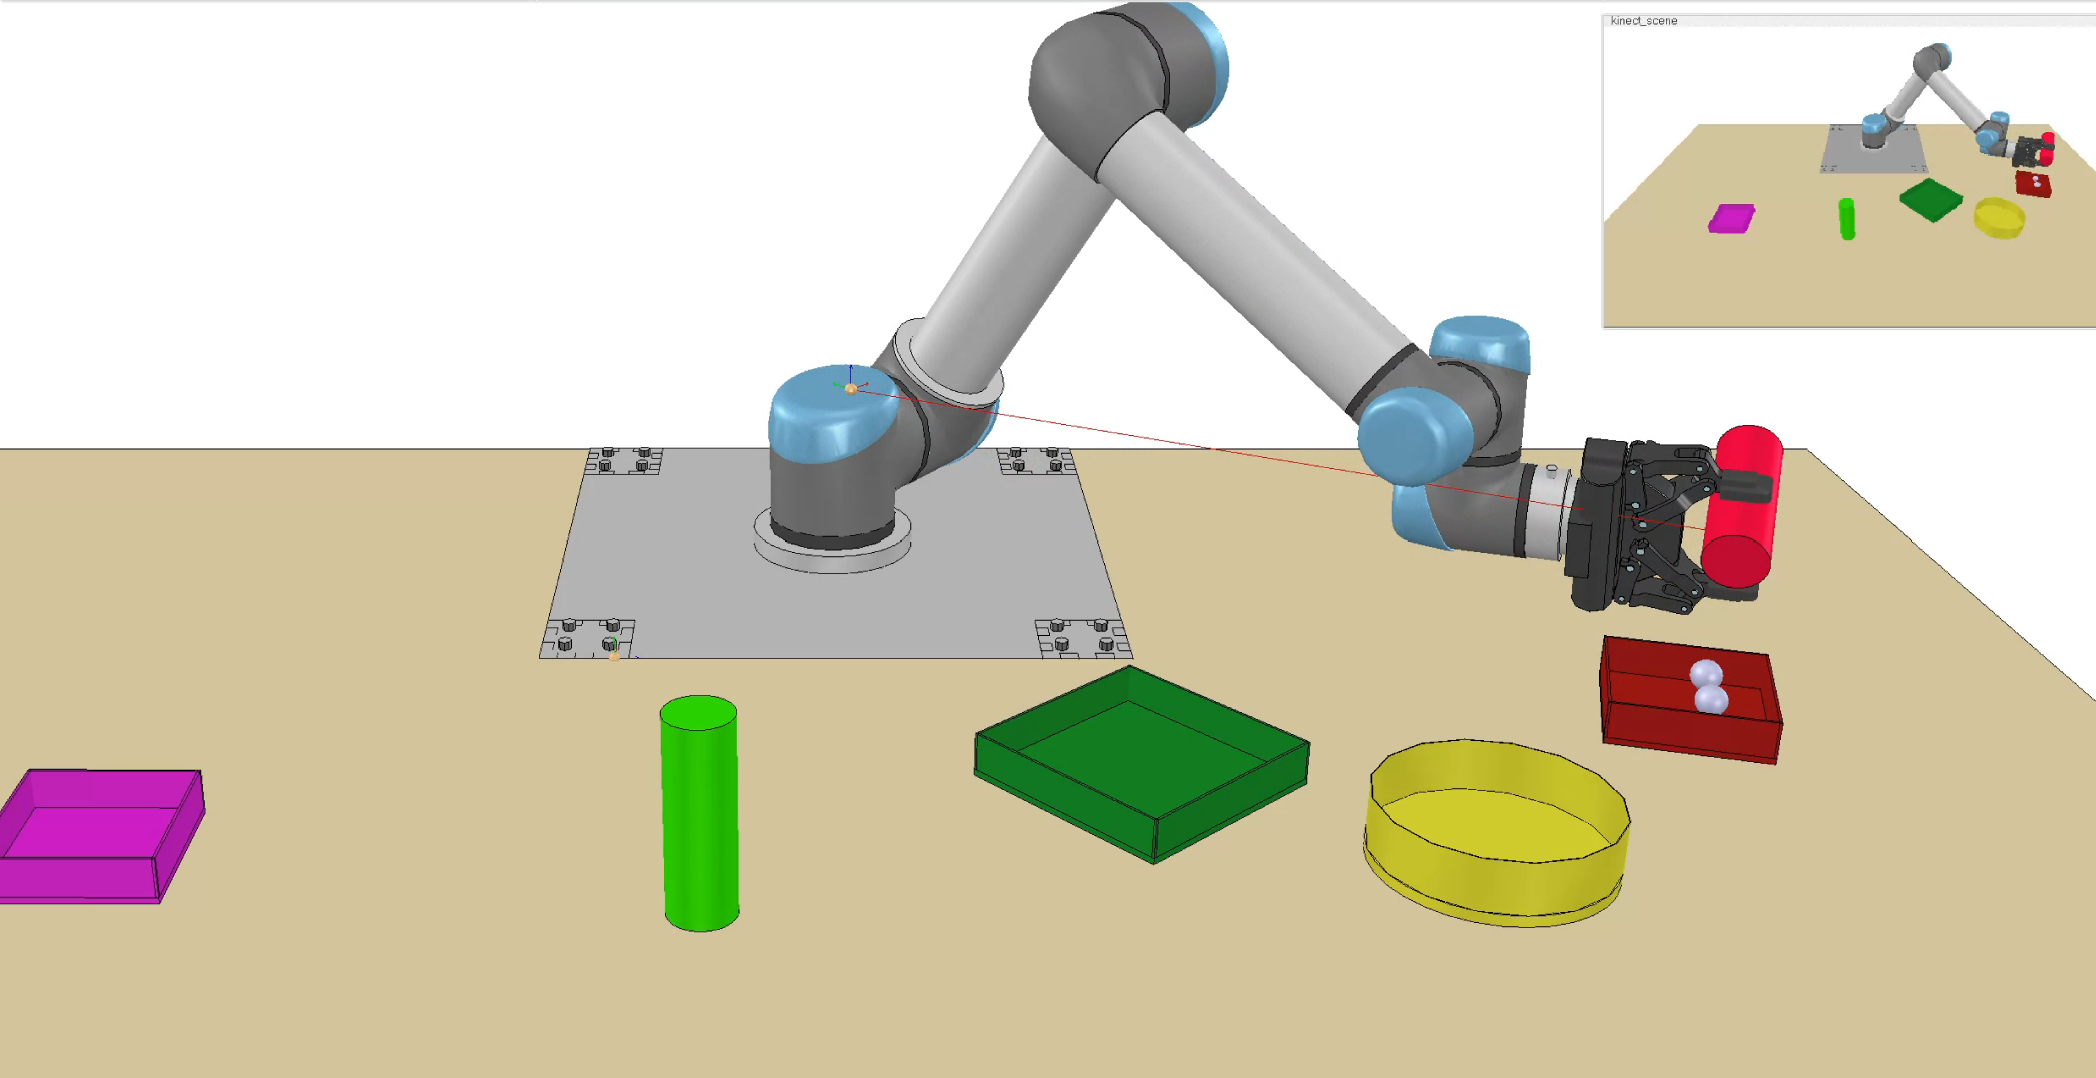
\includegraphics[width=\linewidth]{images/Language_Conditioned_Exp/mine_5.png}
        \caption{Time step 300.}
    \end{subfigure}
    \caption{Comparison of a pour task. Recurrent Policy (top row) spills the content over the table and moves unpredictable. The task is considered a failure 
    by the benchmark, as most drops did not land in the goal bowl. Active Critic (bottom row) performs the task as intendet with no unexpected movement.}
    \label{fig: AC vs. Rec}
\end{figure}
Moreover in figure \ref{fig: AC vs. Rec} we have depicted a case in the test dataset, which our policy solved and compared it to the performce of the recurrent algorithm, which failed at the task. 
While our approach hit the target precisely, the recurrent model was widely off. We assume this is caused by the fact that during inference time, the 
i.i.d. assumption of the input data to the policy is broken. Intuitively, the recurrent policy 
is in a state that it has not seen before and acts slightly different to the expert movement. After some steps, the policy now sees inputs that are vastly 
different then the training distribution, thus it starts to act unpredictable. As argued in section \ref{COD_AC} this is an advantage of our policy, as it 
does not break the i.i.d. assumption.

